
\documentclass[12pt]{elsarticle}

\usepackage{graphicx}
\usepackage{amssymb}
\usepackage{lineno}
\usepackage[utf8]{inputenc}


\begin{document}

\begin{frontmatter}

\title{Análise da situação financeira dos municípios do Estado de Pernambuco}

\author{Breno Rios, Cinthya Lins}

\address{Centro de Informática, Universidade Federal de Pernambuco}

\begin{abstract}
%% Text of abstract
Realizar uma análise financeira dos municípios do Estado de Pernambuco, com o objetivo de identificar os municípios que não conseguem se sustentar com verbas próprias, e de que maneira isso afeta os indicadores socias desses lugares.
\end{abstract}

\begin{keyword}
Pernambuco \sep Finanças \sep Municípios

\end{keyword}

\end{frontmatter}

%%
%% Start line numbering here if you want
%%
% \linenumbers

%% main text
\section{Hipótese}
\text{
A nossa pergunta inicial foi se o equilíbrio nas contas públicas pode impactar em indicadores demográficos e sociais. Quanto afeta indicadores de escolarização, mortalidade e IDHM - Índice de Desenvolvimento Humano do Município?
}

\label{S:1}

\section{Conjunto de dados}
\text{
As bases dados estão disponíveis no portal de dados abertos do Tribunal de Contas de Pernambuco e no Portal da Transparência de Pernambuco, que contém informações sobre as receitas e despesas de cada município do estado. 
}

\section{Análise dos dados}
\text{
Para realizar a análise foi feita a conversão de arquivos no formato XML e KMZ e transformação das bases em Dataframes. Após o pré-processamento dos dados, que consistiu em tratar dados ausentes, remoção de atributos desnecessários e ajuste de tipos, converter código para identificador com melhor significado foi possível iniciar a análise dos dados e realizar a verificação das correlações consideradas importantes para comprovar as hipóteses feitas no trabalho.
}

\subsection{Balanço}
\text{
Foi analisado o balanço geral de cada município subtraindo o total de suas receitas do total de suas despesas no ano de 2017. Pudemos constatar que 20,6\% dos municípios do estado terminaram o ano de 2017 com um déficit de até R\$ 45 milhões de reais.
}

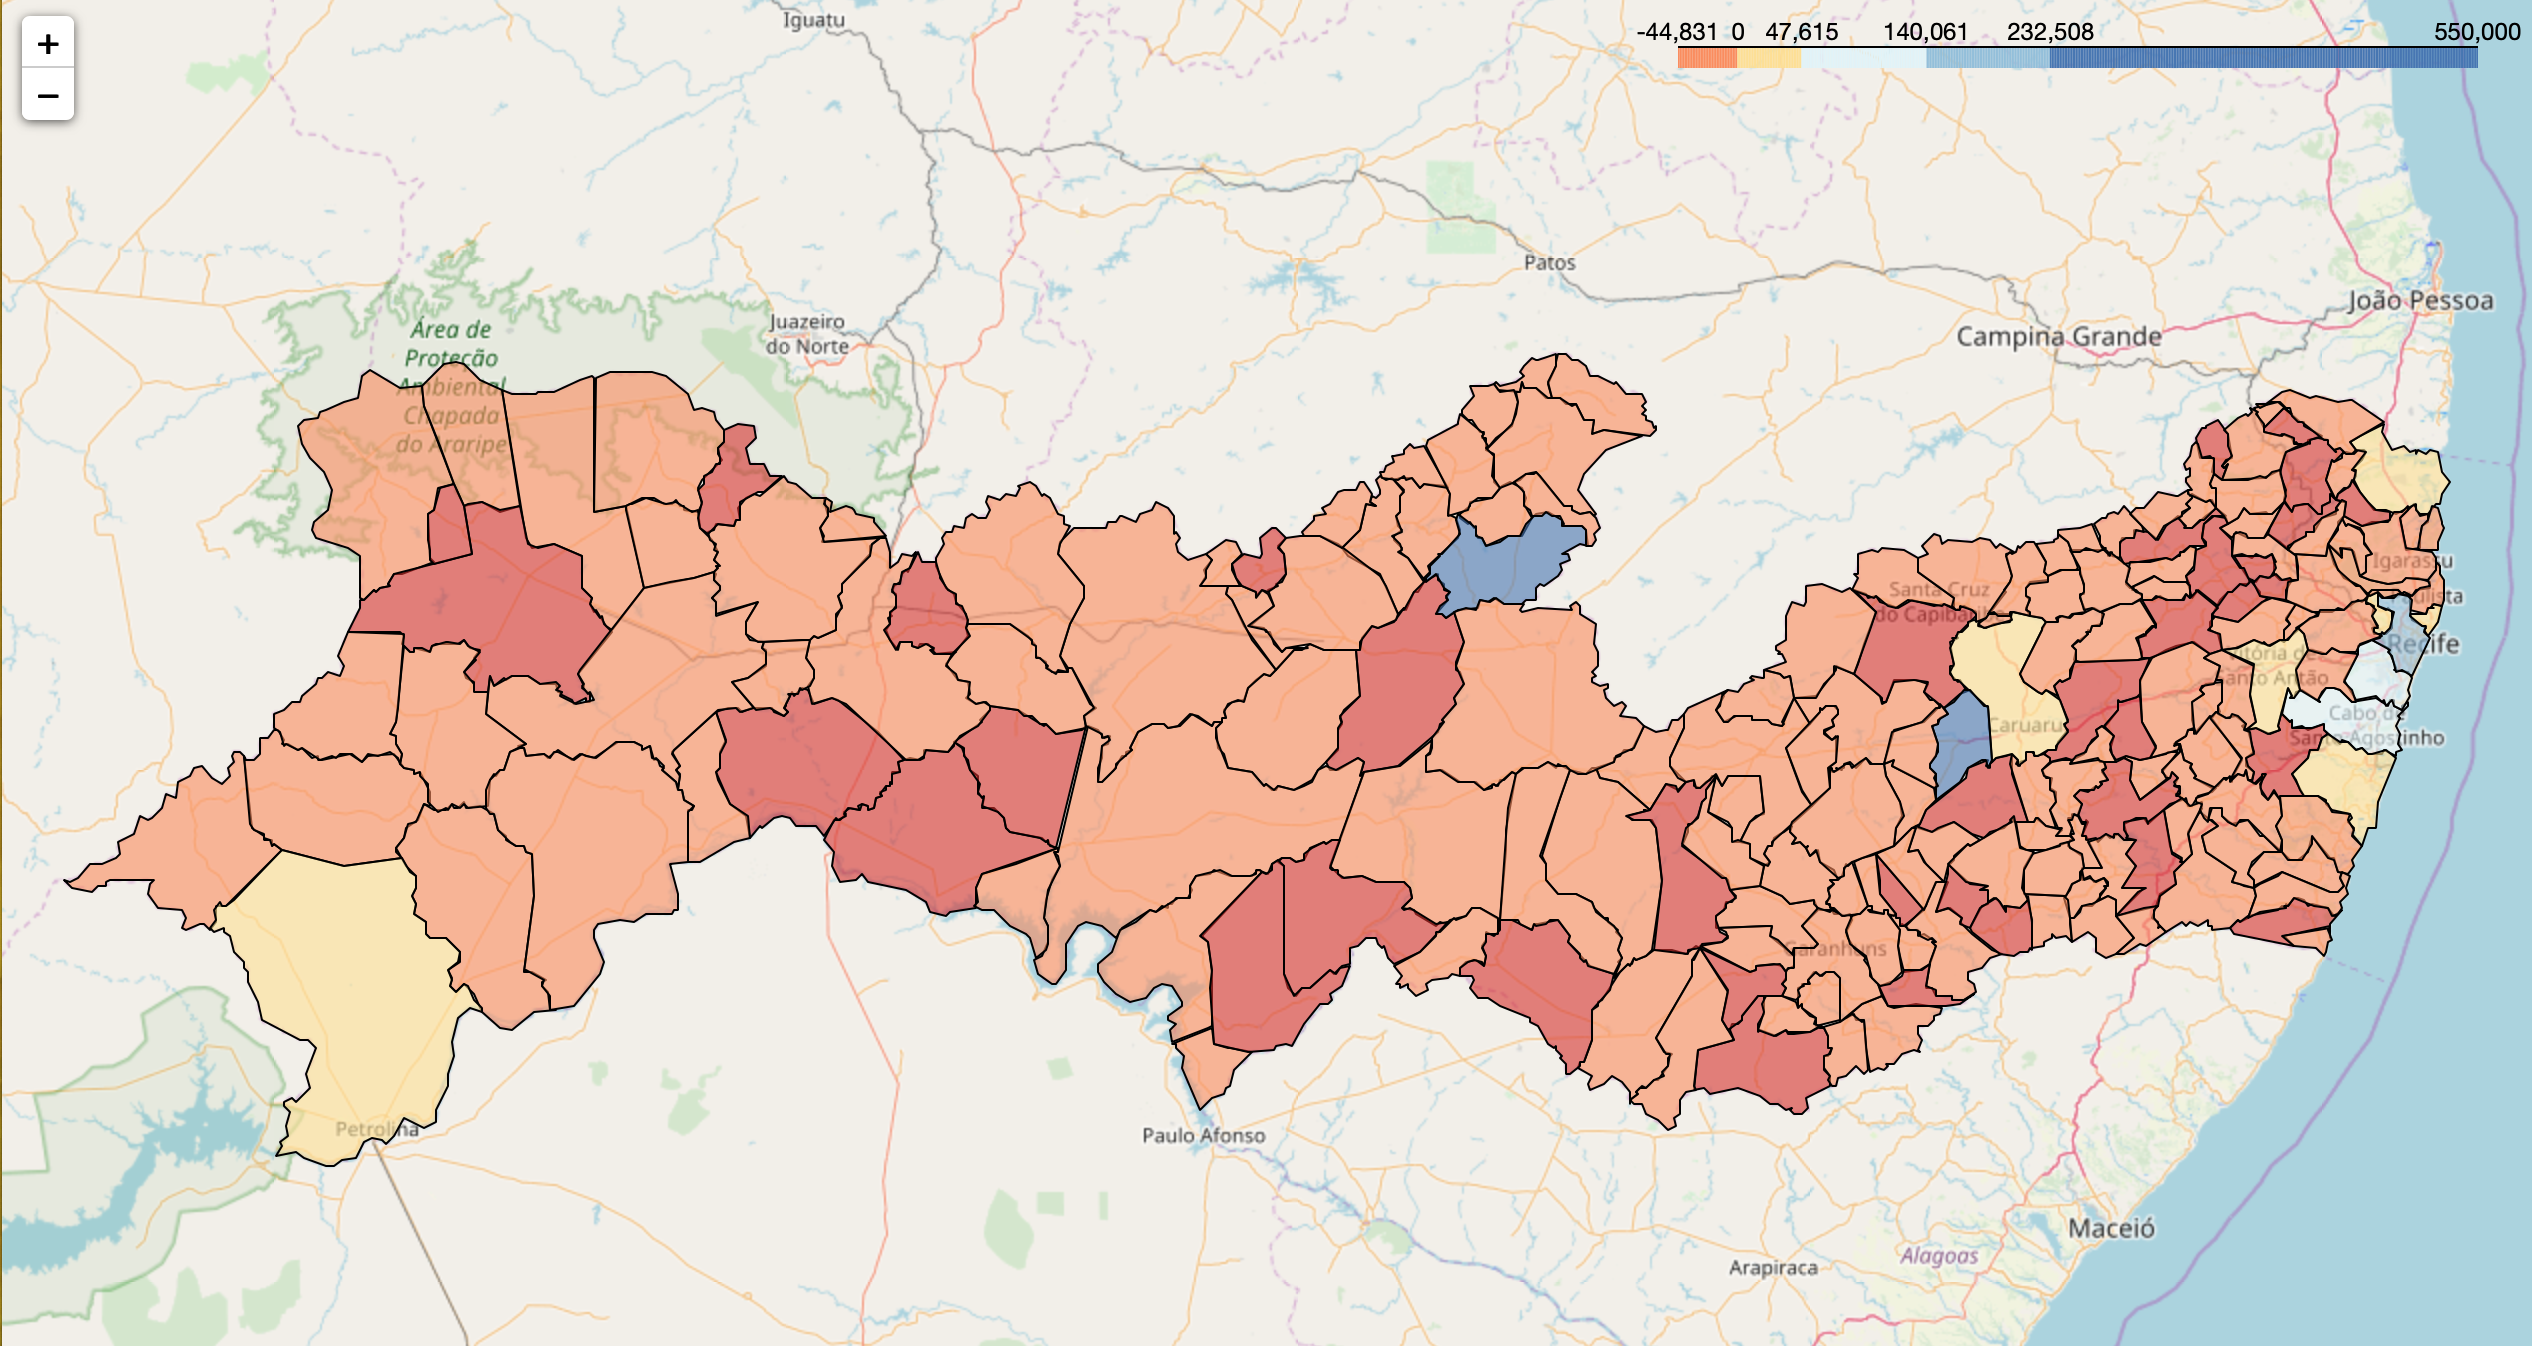
\includegraphics[width=\textwidth]{heat_balanco.png}

\text{
Na média, os municípios pernambucos terminaram 2017 com pouco mais de 10 milhões de reais de superávit. Esse valor é puxado para cima por municípios como Recife (R\$ 504 milhões), Cabo de Santo Agostinho (R\$ 227 milhões) e Jaboatão dos Guararapes (R\$ 223 milhões).
}

\subsection{Mortalidade}
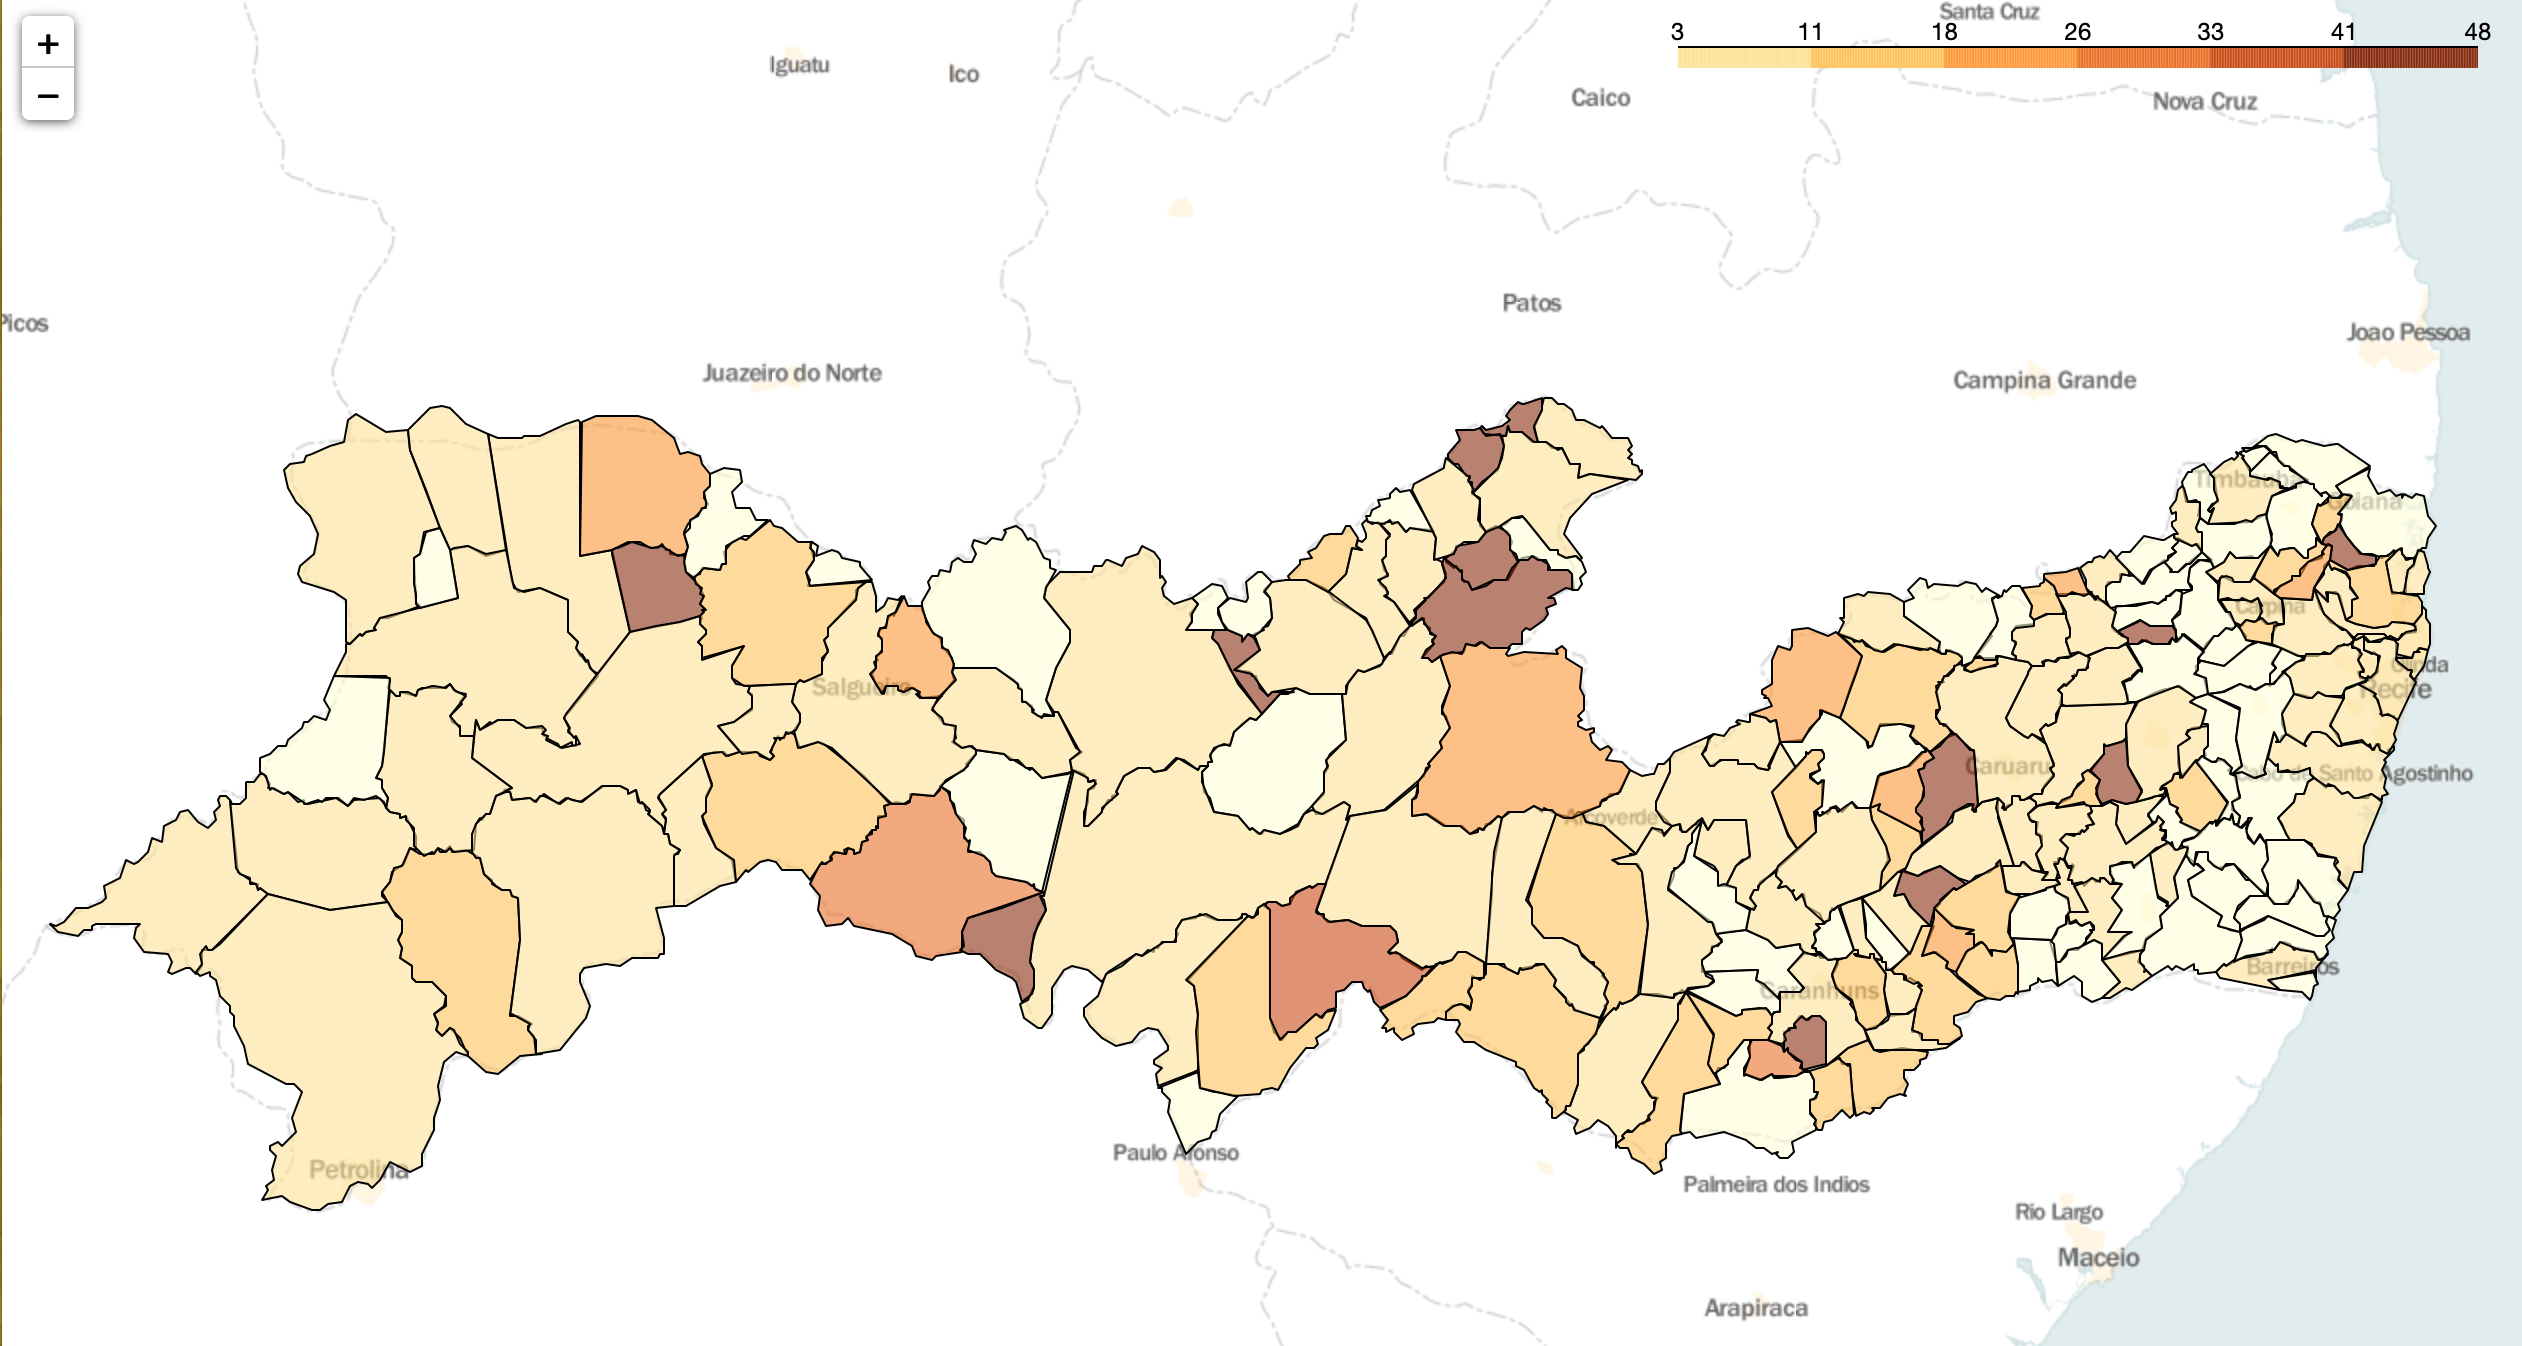
\includegraphics[width=\textwidth]{heat_mortalidade.png}
\subsection{Escolaridade}
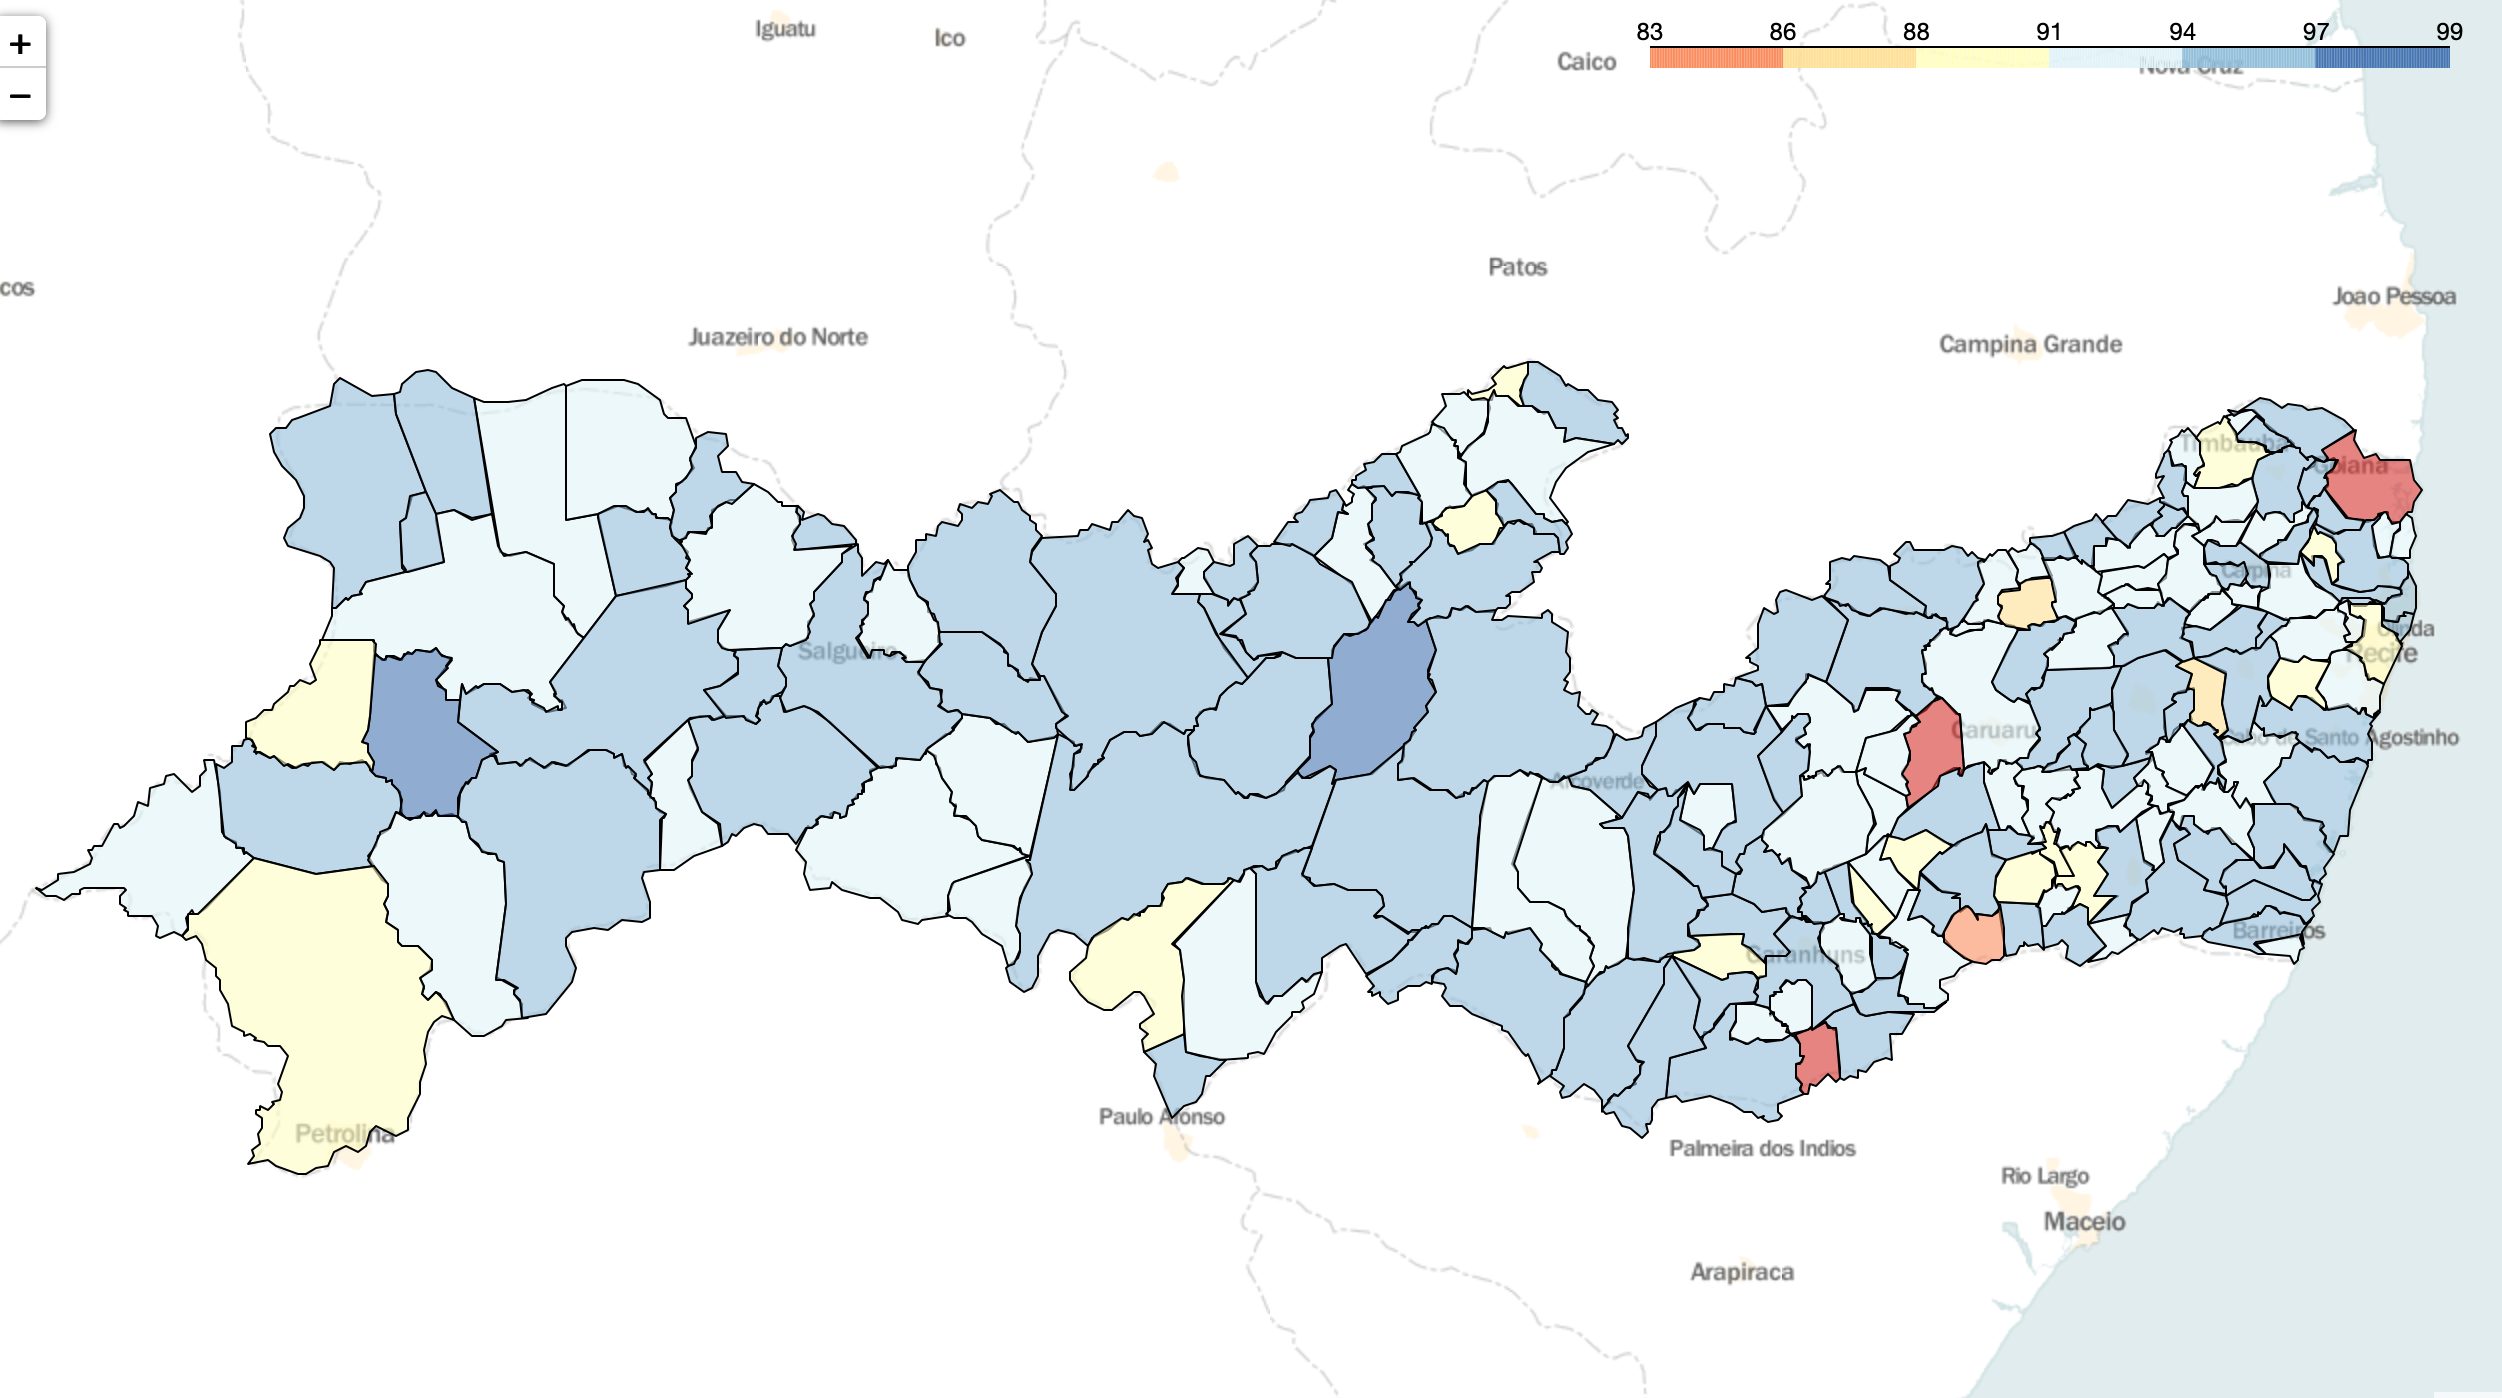
\includegraphics[width=\textwidth]{heat_escolaridade.png}
\text{
Podemos analisar também os mapas de calor dos números de Mortalidade, Escolaridade e IDHM. Aparentemente não há nenhum padrão que possa ser observado.
}
\subsection{IDHM}
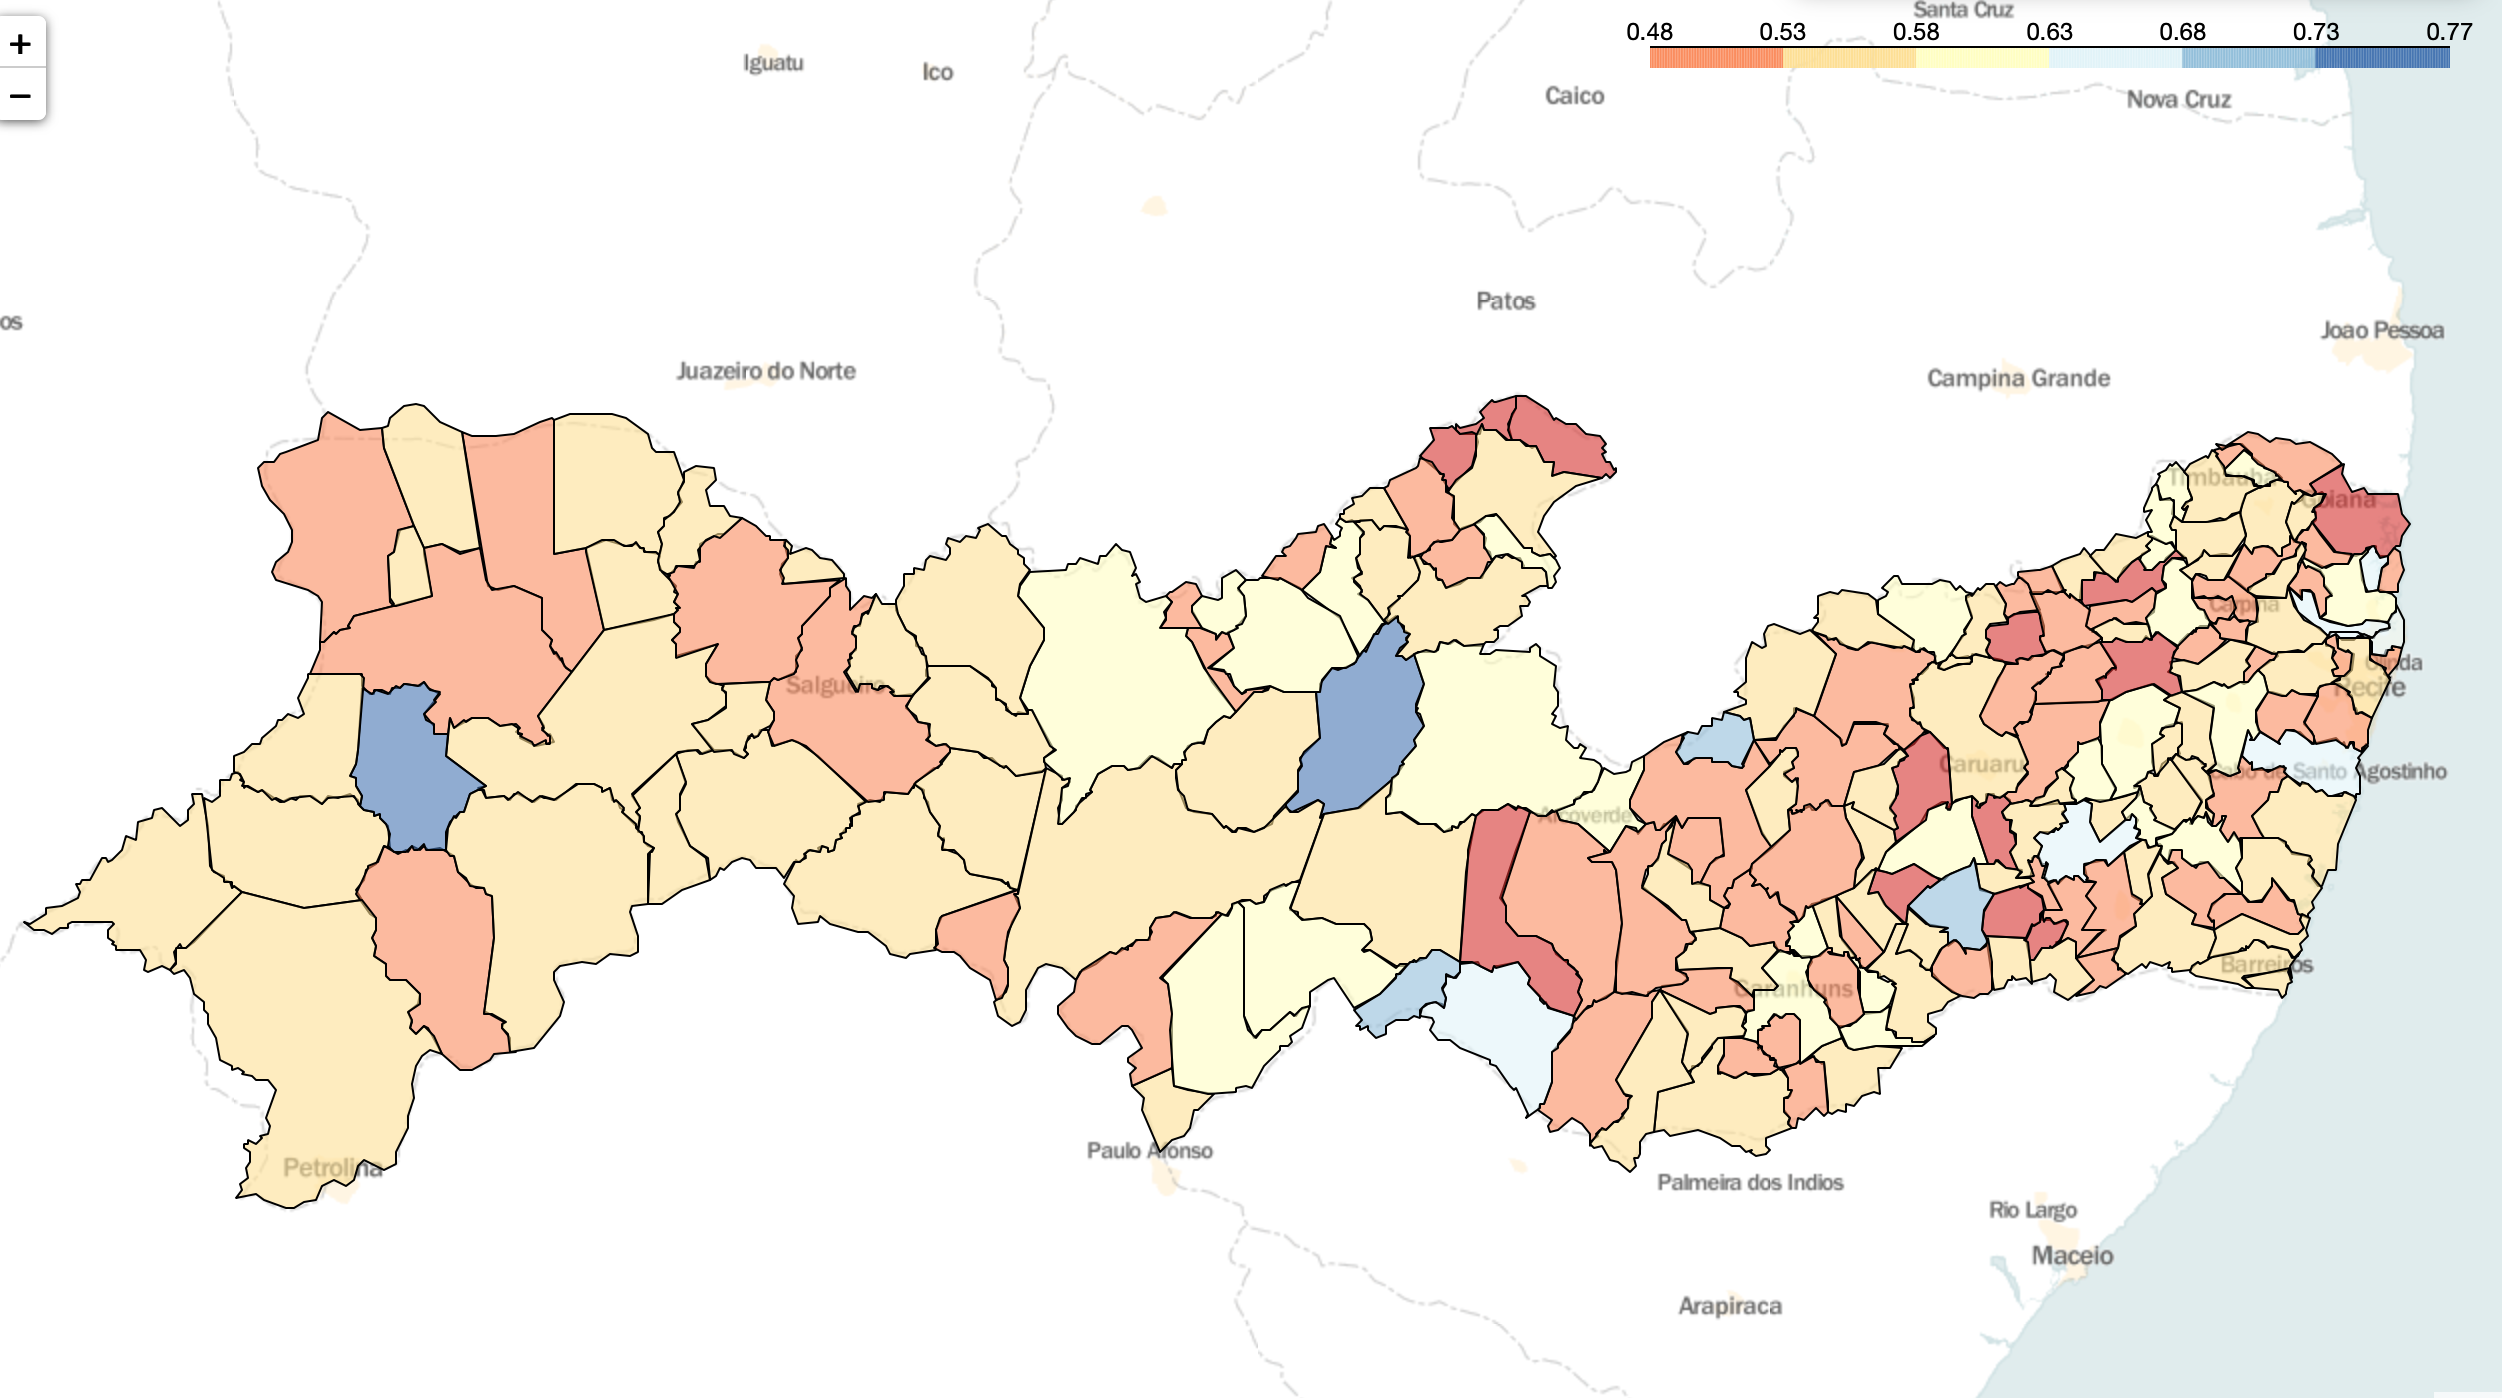
\includegraphics[width=\textwidth]{heat_idhm.png}
\subsection{Correlações}

\text{
Para verificar nossa hipótese inicial, usamos um regressor linear a partir da biblioteca SciPy. Analisamos os valores de p-value, que nos permite constatar se a correlação é forte, e o coeficiente de determinação (R2), que nos dá uma porcentagem do quanto o modelo pode explicar a variância encontrada.
}
\subsubsection{Balanço x IDHM}
\text{
\textbf{R2 = 0.228, p-value=0.000}
Ao analisarmos os parâmetros de balanço e IDHM, vemos um p-value extremamente pequeno, o que indica forte correlação entre os parâmetros. Apesar disso, o modelo usado consegue explicar apenas 22,8\% da variância encontrada.
Como esperado a correlação entre Receitas e Despesas com o IDHM também mostra resultados semelhantes:
\textbf{R2 = 0.226, p-value=0.000}
}
\subsubsection{Balanço x Escolaridade x Mortalidade}
\text{
As análises feitas entre os valores de Balanço e seu impacto na Escolaridade e Mortalidade mostram o que os mapas de calor acima já parecia nos dizer: a correlação é baixíssima entre esses parâmetros. O regressor retornou os valores de \textbf{r2 = 0.001 e p-value=0.619} para a análise Balanço x Mortalidade, mostrando a baixa correlação entre eles. O mesmo ocorreu com os valores para Balanço x Escolaridade \textbf{R2 = 0.003, p-value=0.458}.
}
\text{Não ficou provada a correlação, sendo encontrados R2 = 0.001, p-value=0.619}
\subsubsection{Receita x Mortalidade}
\text{Não foi provada correlação, sendo R2 = 0.003, p-value=0.458 }
\subsubsection{Despesa x Mortalidade}
\text{Não foi provada correlação, sendo obtidos os seguintes valores na análise: R2 = 0.002, p-value=0.540 }
\subsubsection{Despesa x Escolaridade x Receita}
\text{
Outras correlações também foram analisadas, mas não mostraram também um valor alto para o p-value e baixo para o R2. Seguem seus valores abaixo:
}
\text{Despesa x Escolaridade: \textbf{R2 = 0.004, p-value=0.437}}
\text{Receita x Escolaridade: \textbf{R2 = 0.004, p-value=0.436}}

\subsubsection{IDHM x Mortalidade x Escolaridade}
\text{Como esperado, a correlação entre IDHM e Mortalidade, assim como Escolaridade apresenta correlação de acordo com os valores obtidos: IDHM x Mortalidade \textbf{R2 = 0.044, p-value=0.005}, IDHM x Escolaridade \textbf{r2 = 0.103, p-value=0.000}. Isso ocorre pois os números de Mortalidade e Escolaridade contribuem para o cálculo do IDHM.
}

\section{Conclusão}
 Pudemos concluir que os municípios que terminaram o ano com um superávit tendem a ter um IDHM maior. Outra coisa interessante de se notar é que as Receitas ou as Despesas não são fatores que influenciam diretamente na Escolaridade e Mortalidade.

\section{Referências}
\begin{thebibliography}{00}

\bibitem .Dados sobre as receitas e despesas de cada ano divididos por Unidades Gestoras. Tribunal de Contas de Pernambuco (2018). https://www.tce.pe.gov.br/internet/index.php/dados-abertos/bases-de-dados-completas 
\bibitem Arquivos com os limites geográficos de cada município. Gmapas. http://www.gmapas.com/poligonos-ibge/poligonos-municipios-ibge-pernambuco
\bibitem .Dados sobre a posição geográfica das sedes dos municípios. Base de dados do Estado. http://www.bde.pe.gov.br/visualizacao/Visualizacao\underline{\space}formato2.
aspx?codFormatacao=703&CodInformacao=280&Cod=1
\bibitem .Dados demográficos de cada município de Pernambuco. Instituto Brasileiro de Geografia e Estatística. https://www.ibge.gov.br/estatisticas-novoportal/por-cidade-estado-estatisticas.html?t=destaques&c=26
\bibitem .Dados demográficos de cada município de Pernambuco. Base de dados do Estado.
http://www.bde.pe.gov.br/site/ConteudoRestrito2.aspx?
codGrupoMenu=84&codPermissao=5
\bibitem .Dados sobre as despesas do Estado de Pernambuco. Portal da tranparência de Pernambuco. http://web.transparencia.pe.gov.br/dados-abertos/   
\end{thebibliography}


\end{document}
